\chapter{Overview of Tool}\label{sec:swinstruct}

\section{Interface}
The interface of the program is based on two parts.  First, a command line
interface (CLI) where input and output is handled.  Second, a graphical
presentation of images, using the matplotlib library in Python which allows for
plotting several images in the same area.

Eg. the CLI simply looks like the following snippet below.  While the graphical
display of images is shown in figure \ref{fig:gui_display}.
The CLI is controlled through very specifically formatted commands and responses
from queries by the system.
\lstinputlisting{chapters/appendices/menu.txt}
\begin{figure}[h]
	\center
	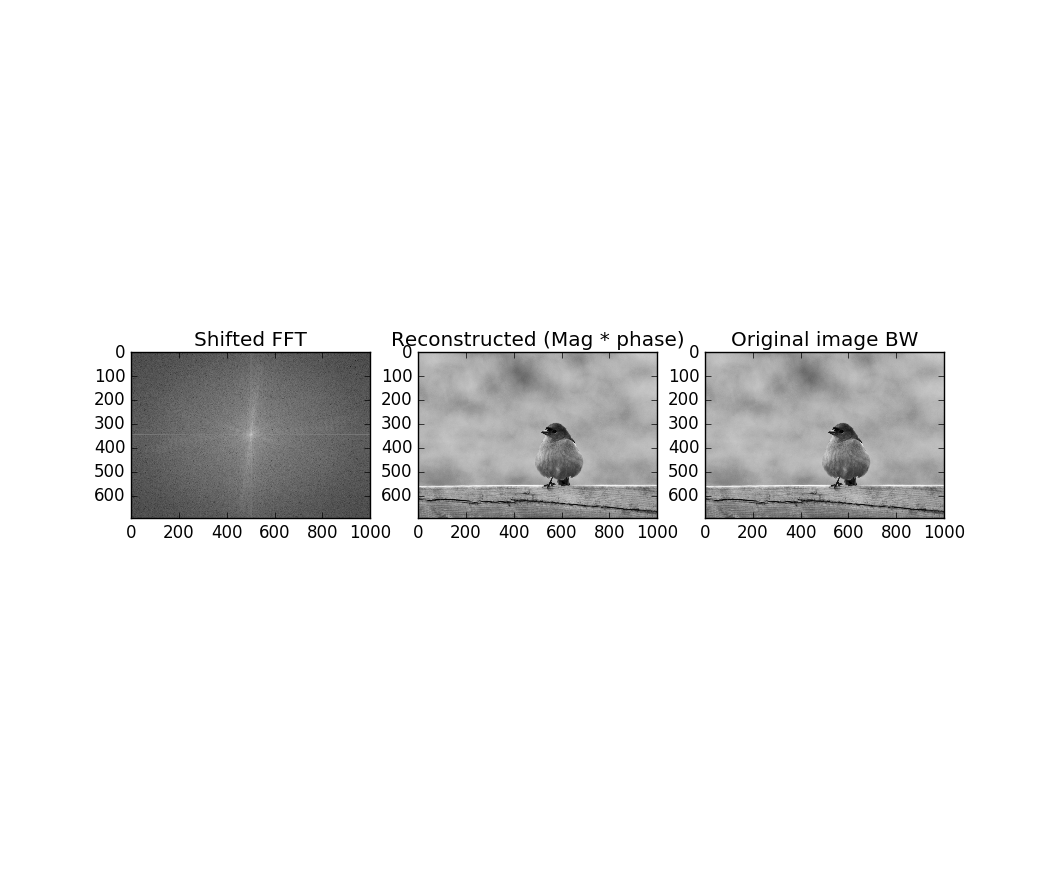
\includegraphics[width={1\linewidth},trim={50px 235px 50px 230px},clip]{pics/gui_display}
	\caption{Graphical visualisation of images}\label{fig:gui_display}
\end{figure}


\section{Comparison Metrics}
The comparison regime installed in this application is based on the evaluation
of histogram data of the image which is being compared.  The computations are
collected from some of the mentioned methods in the paper by Meshgi and Ishii,
"Expanding histogram of colours with gridding to improve tracking
accuracy"\cite{histMetrics}.  Root Mean Squared Error (RMSE) is the third metric
calculated. The chosen metrics are very small subset of metrics that could be
calculated, and more are proposed at the end of the conclusion, as future work
proposals. Among the more interesting metrics could be natural scene statistics,
focus assessment, feature detection, and contrast levels.

In addition to the metrics, during comparison the histogram for both the
original image and the altered image is calculated. A third histogram is
generated by calculating the absolute difference between each of the points in
the histograms, giving a histogram of the differences between the images for
visual inspection. In summation, the comparison metrics being generated in the 
application are the following metrics.
\begin{multicols}{3}
\begin{itemize}
	\item Manhattan Distance
	\item Euclidean Distance
	\item Root Mean Squared Error
	\item Histogram
	\item Histogram difference
\end{itemize}
\end{multicols}


\paragraph{Manhattan Distance}
Manhattan distance is a commonly used metric for measuring the difference
between two values. It takes the sum of each value in the histogram of the
histogram belonging to the altered histogram $H_b$ and subtracts it from the
same value original histogram $H_a$.  The absolute value is calculated from the
resulting answer and the total difference for the entire histogram is summed.
Two completely equal images should yield difference of $0$.
\begin{align}
	D_{manhattan} &= \Sigma^{n=255}_{i=0} | H_{a}(x,y) - H_{b}(x,y) |
\end{align}


\paragraph{Euclidean Distance}
Euclidean is quite similar to Manhattan distance, but the root of the result
from the Manhattan Distance metric is calculated. Giving us the Euclidean
distance metric, as shown below.
\begin{align}
	D_{euclid} &= \sqrt{\Sigma^{n=255}_{i=0} (H_a(x) - H_b(x,y))^2}
\end{align}


\paragraph{Root Mean Squared Error}
The RMSE first generates a new matrix of MxN size, which contains the squared
product of subtracting the original histogram from the altered version. This
gives us the $H_{diff}$, as shown below.
The mean value of $H_{diff}$ is then calculated and the root of the mean value
is taken, giving us the value of RMSE.
\begin{align}
	H_{diff} &= (H_b - H_a)^2 \\
	RMSE &= \sqrt{ mean( H_{diff} ) } 
\end{align}


\paragraph{Histogram}
The histograms are generated by going through the image in the spatial domain
and enumerating the instances of each grey scale value, shown in the equation
below.  The histogram works as the initial point for calculating the above
metrics, but is also used by the program to visualise the distribution of gray
levels in original vs. altered image when running the comparison functionality.
The differentiation between altered and original image is shown in its own
histogram with better resolution where the absolute difference between them are
visualised.
\begin{align}
	H_i = H_i + 1 | \forall_y\forall_x f(x,y) = i
\end{align}


\section{Image Operations}
There are several image operations available to be performed on the image, but
not implemented directly for the user to choose. When an image has a set of
actions performed on it, the procedure for reverting it to the original state or
representation state is stored along the image, making it possible to operate in
the Fourier spectrum and reverting it to the spatial domain automatically. The 
available set of functions to perform on the image is the following, where the
index number refers to the index of the operation in the program.
\begin{enumerate}
	\item[0.] ABS: Return the absolute values in the matrix. $|f(m,n)|$.
	\item IFFT2: Performs the inverse 2D fast Fourier Transform. $\Im^{-1}$.
	\item IFFTSHIFT: Performs the inverse operation of shifting the Fourier
		spectrum.
	\item Log: Returns the logarithmic representation of the Fourier spectrum.
		$\log(1+\Im)$.
	\item[10.] FFT2: Transforms the image from spatial representation to frequency
		representation using the 2D Fast Fourier Transform. $\Im( f(x,y) )$.
	\item[11.] FFTSHift: Shifts the Fourier transform, so the centre of the
		frequency spectrum contains the low frequencies and high frequencies are
		located at the edges.
	\item[12.] Real: Returns the real part of the Fourier spectrum. 
		$R = real(\Im(f(x,y)))$.
	\item[13.] Imaginary: Returns the imaginary part of the Fourier spectrum.
		$I = imag(\Im(f(x,y)))$
	\item[14.] Phase: Calculates and returns the phase values of the image in the
		Fourier spectrum. $\rho=\exp(1j*angle(\Im))$.
	\item[15.] Magnitude: Calculates and return the magnitude representation of
		the Fourier transform. $M=|\Im|$.
\end{enumerate}

\section{Additional functionality}
In addition to the previously mentioned abilities in the program there are
several extra features built in to the program.  Among others are that the
database is arbitrary and can take any image and perform the actions on it, 
given that it's either "JPEG", "BMP", "TIFF" or "PNG" formatted.

The images can be saved, either upon exiting the software or explicitly telling
the program to save the selected images.  This will save the image as a "JPEG"
formatted image in the "./outdir" and a text file containing the metric data
belonging to the image.




\chapter{Filters}
In this application I have focused on five types of filters. These consists of
low pass filters, high-pass filters, line filters and spot detection filters.
Below are the different filters available in the application listed. These
filters are further explained later on. 
\begin{multicols}{3}
\begin{itemize}
	\item Low-Pass Filter
	\begin{itemize}
		\item[$\circ$] Ideal Kernel
		\item[$\circ$] Gaussian Kernel
		\item[$\circ$] Butterworth Kernel
	\end{itemize}

	\item High-Pass Filter
	\begin{itemize}
		\item[$\circ$] Ideal Kernel
		\item[$\circ$] Gaussian Kernel
		\item[$\circ$] Butterworth Kernel
	\end{itemize}

	\item Line Rotation Filter
	\item Vertical \&\ Horizontal Line Filter
	\item Spot Detection Filter
\end{itemize}
\end{multicols}


\section{Low Pass Filter}
\begin{figure}[h]
\begin{minipage}{0.57\linewidth}
	This filter has three separate sub-types for generating the kernels method of 
	applying the cut-off frequency.  A low pass filter will block out everything
	in the image, except for the low frequencies in the Fourier transformed image.
	This means that it, for a shifted Fourier spectrum will allow all frequencies
	from the centre and to the cut-off frequency ($D0$) to be viewed.  This is
	shown in fig \ref{fig:lp_ideal} where the centre allows the Fourier spectrum
	to pass through while the rest of the Fourier spectrum is blocked by the
	binary mask.

	Fig \ref{fig:lp_ideal} shows the ideal low-pass filtering method where the
	cut-off frequency drops from one, directly to 0.
\end{minipage}\hfill
\begin{minipage}{0.4\linewidth}
	\centering
	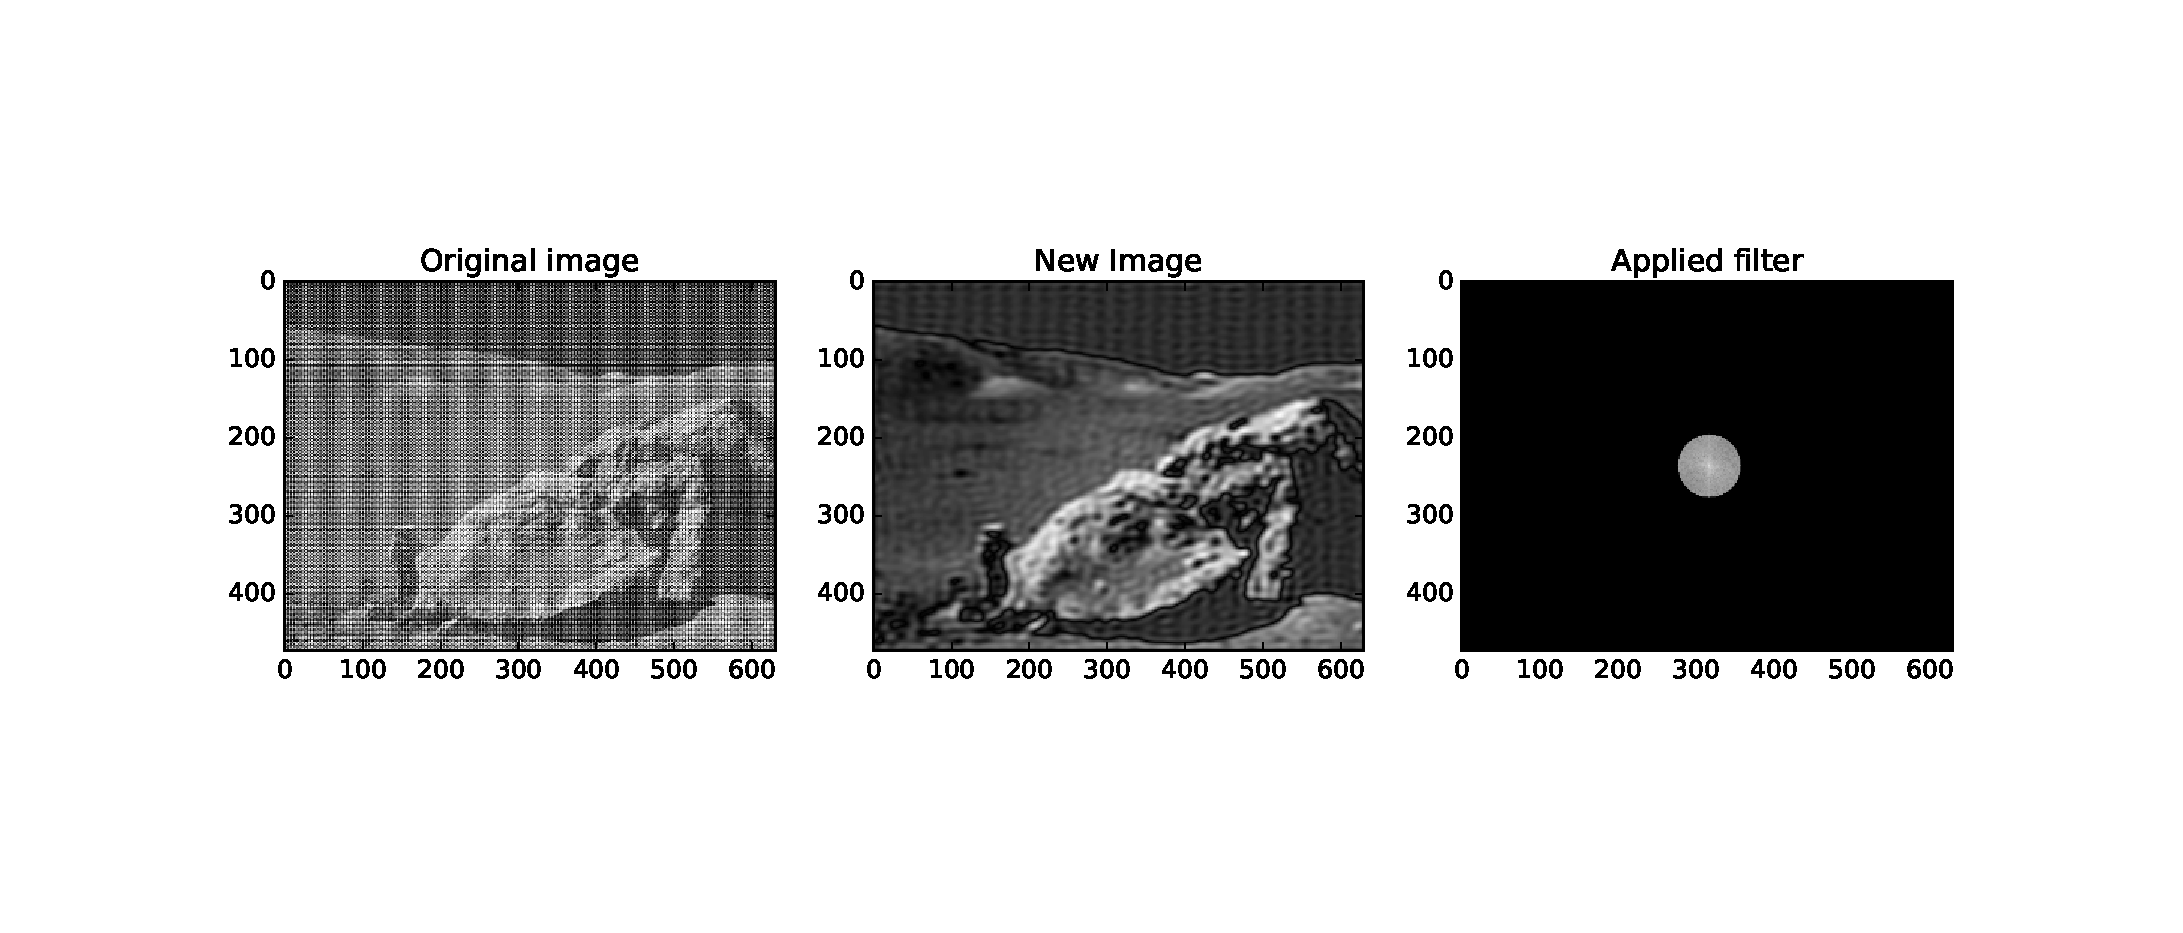
\includegraphics[width=1\linewidth,clip,trim={650 110 75 110}]{pics/moon_lp_ideal}
	\caption{Ideal Low Pass Filter applied to Shifted Fourier Transform}
	\label{fig:lp_ideal}
\end{minipage}
\end{figure}

\pagebreak
\section{High Pass Filter}
\begin{figure}[h]
\begin{minipage}{0.57\linewidth}
	In the basic definition an high-pass filter is the direct inverse of an
	low-pass filter.  The high-pass filter allows all frequencies from the cut-off
	frequency ($D0$) and outwards to be displayed, and all frequencies lower than
	the cut-off value will be blocked based on the filter method.

	A big difference when using the high-pass filter all low frequencies are
	filtered out.  So to use the high-pass filter to sharpen an image we have to 
	use it as a boost and add it to the existing image.  The result is a new image
	with more intense high-frequencies.

	Fig \ref{fig:hp_ideal} shows the ideal high-pass filtering method where the
	cut-off frequency drops from one, directly to 0.  The filter is then added tot
	the original filter by a multiplicative value, $k\ge1.0$.
\end{minipage}\hfill
\begin{minipage}{0.4\linewidth}
	\centering
	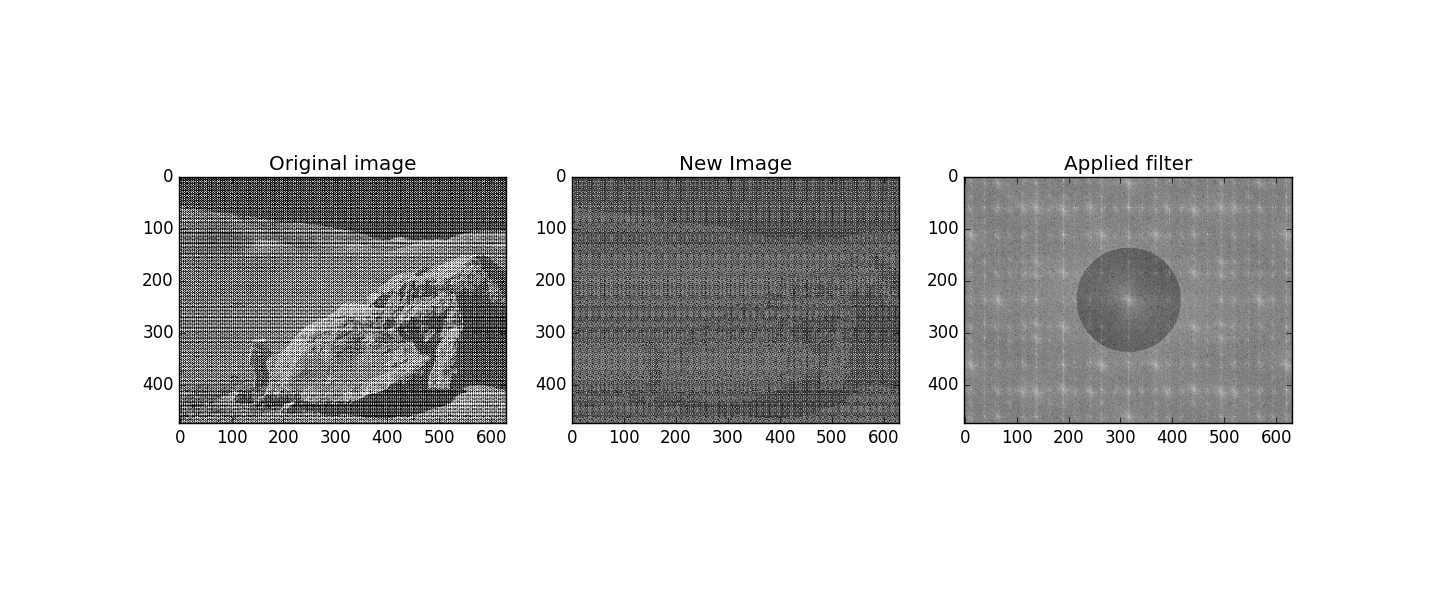
\includegraphics[width=1\linewidth,clip,trim={650 110 75 110}]{pics/moon_hp_ideal}
	\caption{Ideal High Pass Filter applied to Shifted Fourier Transform, with k=5}
	\label{fig:hp_ideal}
\end{minipage}
\end{figure}


\section{Line Rotate filter}
\begin{figure}[h]
\begin{minipage}{0.57\linewidth}
The following filter generates a line filter for assessing and filtering out
specific lines emerging from the centre and outwards in the shifted Fourier
spectrum. It is achieved by creating a line at $0^\circ$, from the offset equal
to the cut-off frequency ($D0$) and out.  This line filter is then rotated for
every $0.5^\circ$ and the local mean is compared to the mean of the MxN matrix.
If the local mean is greater than desired the line is blocked.

The resulting filter is shown in figure \ref{fig:fltr_line_rotate}.  This filter
has a severe drawback because at an angle different than $0^\circ$ or
$180^\circ$ the lines will not reach the all the way to the end of the matrix.
\end{minipage}\hfill
\begin{minipage}{0.4\linewidth}
	\centering
	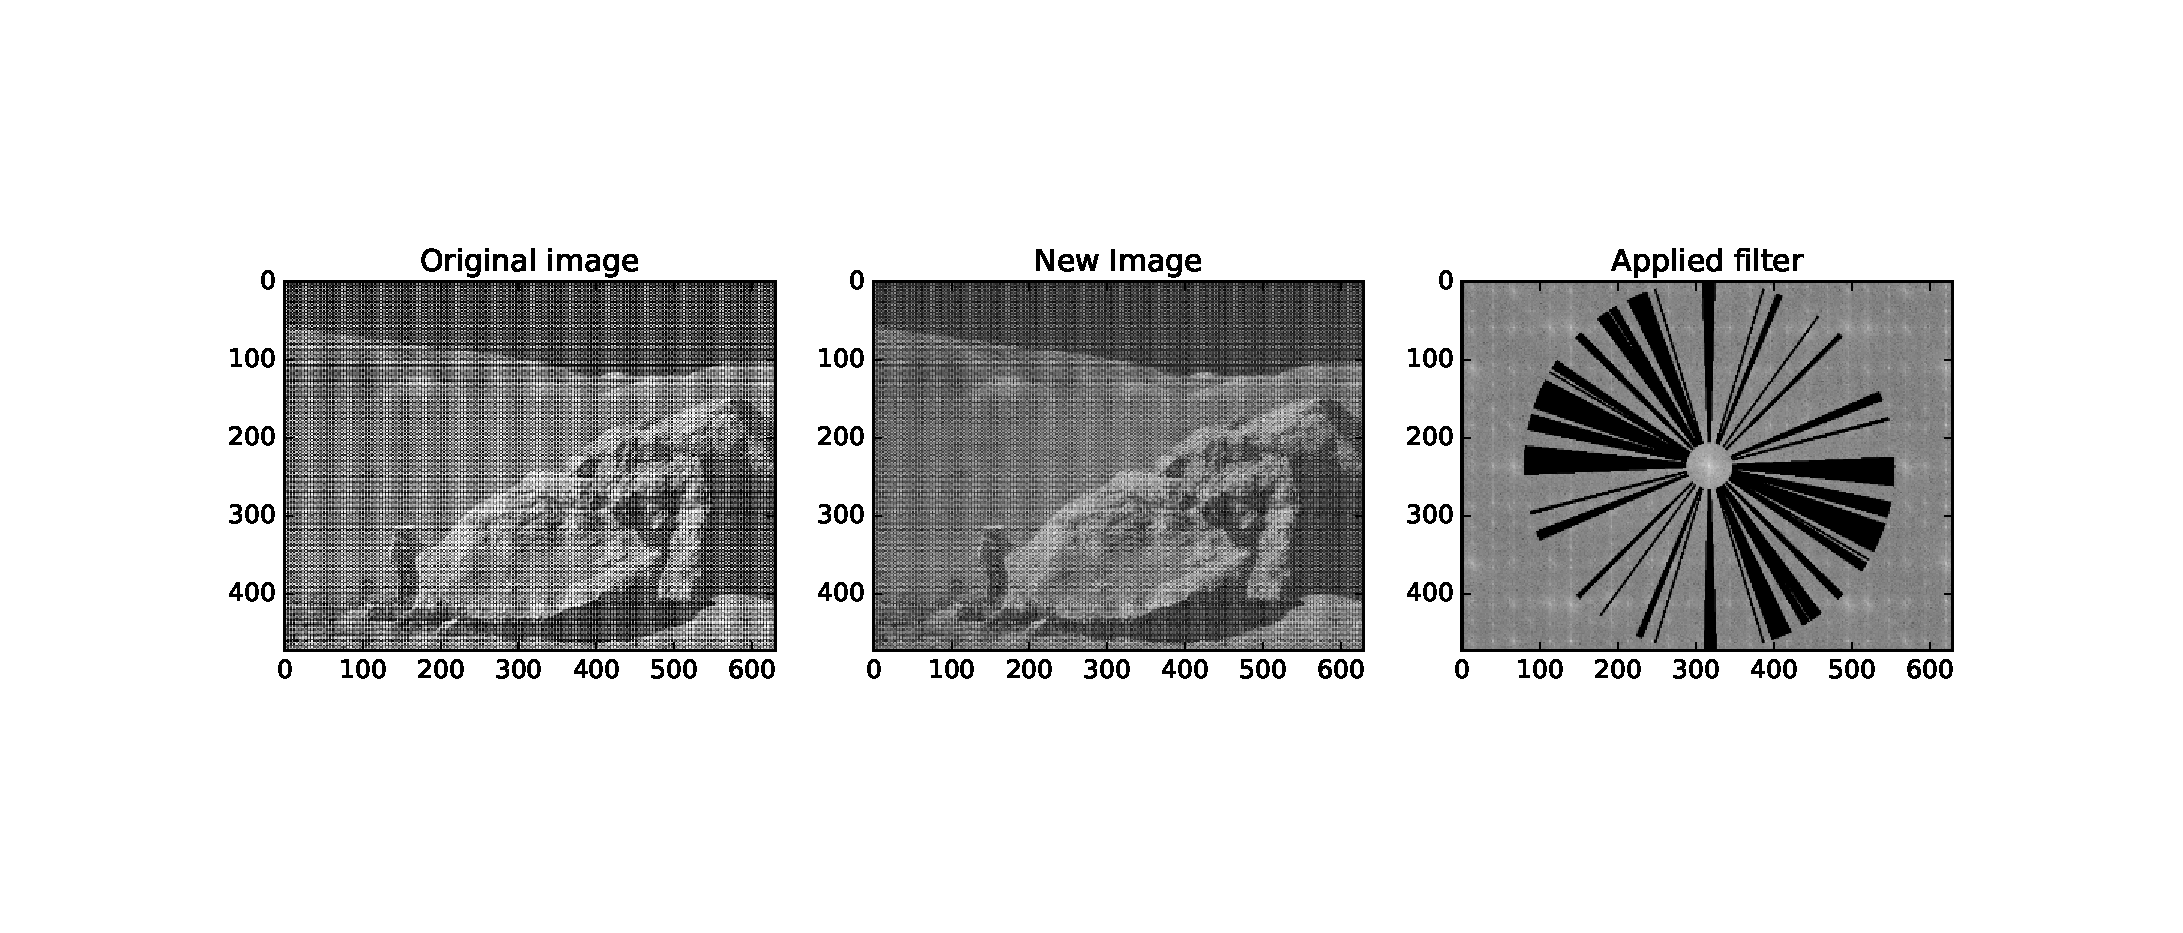
\includegraphics[width=1\linewidth,clip,trim={650 110 75 110}]{pics/moon_fltr_line_rotate}
	\caption{Filter for removing lines emerging from the centre of the Fourier
	Spectrum}
	\label{fig:fltr_line_rotate}
\end{minipage}
\end{figure}



\section{High Energy Spot Filter}
This filter bases itself on comparing the local mean of the subset being checked
to the mean of the entire picture. The idea of this filter is to discover
high energy spots in the Fourier Spectrum and filter them out.

The filter checks five pixels in a 3x3 subset of the MxN matrix which is the
Fourier Spectrum. It takes the mean of the four direct neighbouring pixels and
itself, then compare it to the mean of the MxN matrix.  If the local mean is
greater than the total mean multiplied by the threshold value $k>0.0$, the
centre pixel ($f(x,y)$) is marked as being blocked ($f(x,y)=0$) in the filter $H$.

The resulting Fourier Spectrum after applying the filter the original Fourier
transform is shown below, figure \ref{fig:fltr_spot}.

\begin{figure}[h]
\begin{minipage}{0.57\linewidth}
The filter is generated as described above by comparing the local mean against
the global mean value of the Fourier spectrum. Then, the 2D filter matrix of
MxN size, is for each pixel $[x,y]$ set either as being  $0$ if the comparison
is fulfilled. The comparison is fulfilled when:
\begin{align}
	H_{x,y} &= [\substack{1 if Mean_{local} > (Mean_{global} * k)\\
											 0 if Mean_{local} \le (Mean_{global} * k)}
\end{align}
In the end I've generate a low pass filter with an "ideal" cut-off and add it to
the generated filter $H$.  The source code for this filter is shown in the 
appendix, \ref{code:spot}.
\end{minipage}\hfill
\begin{minipage}{0.4\linewidth}
	\centering
	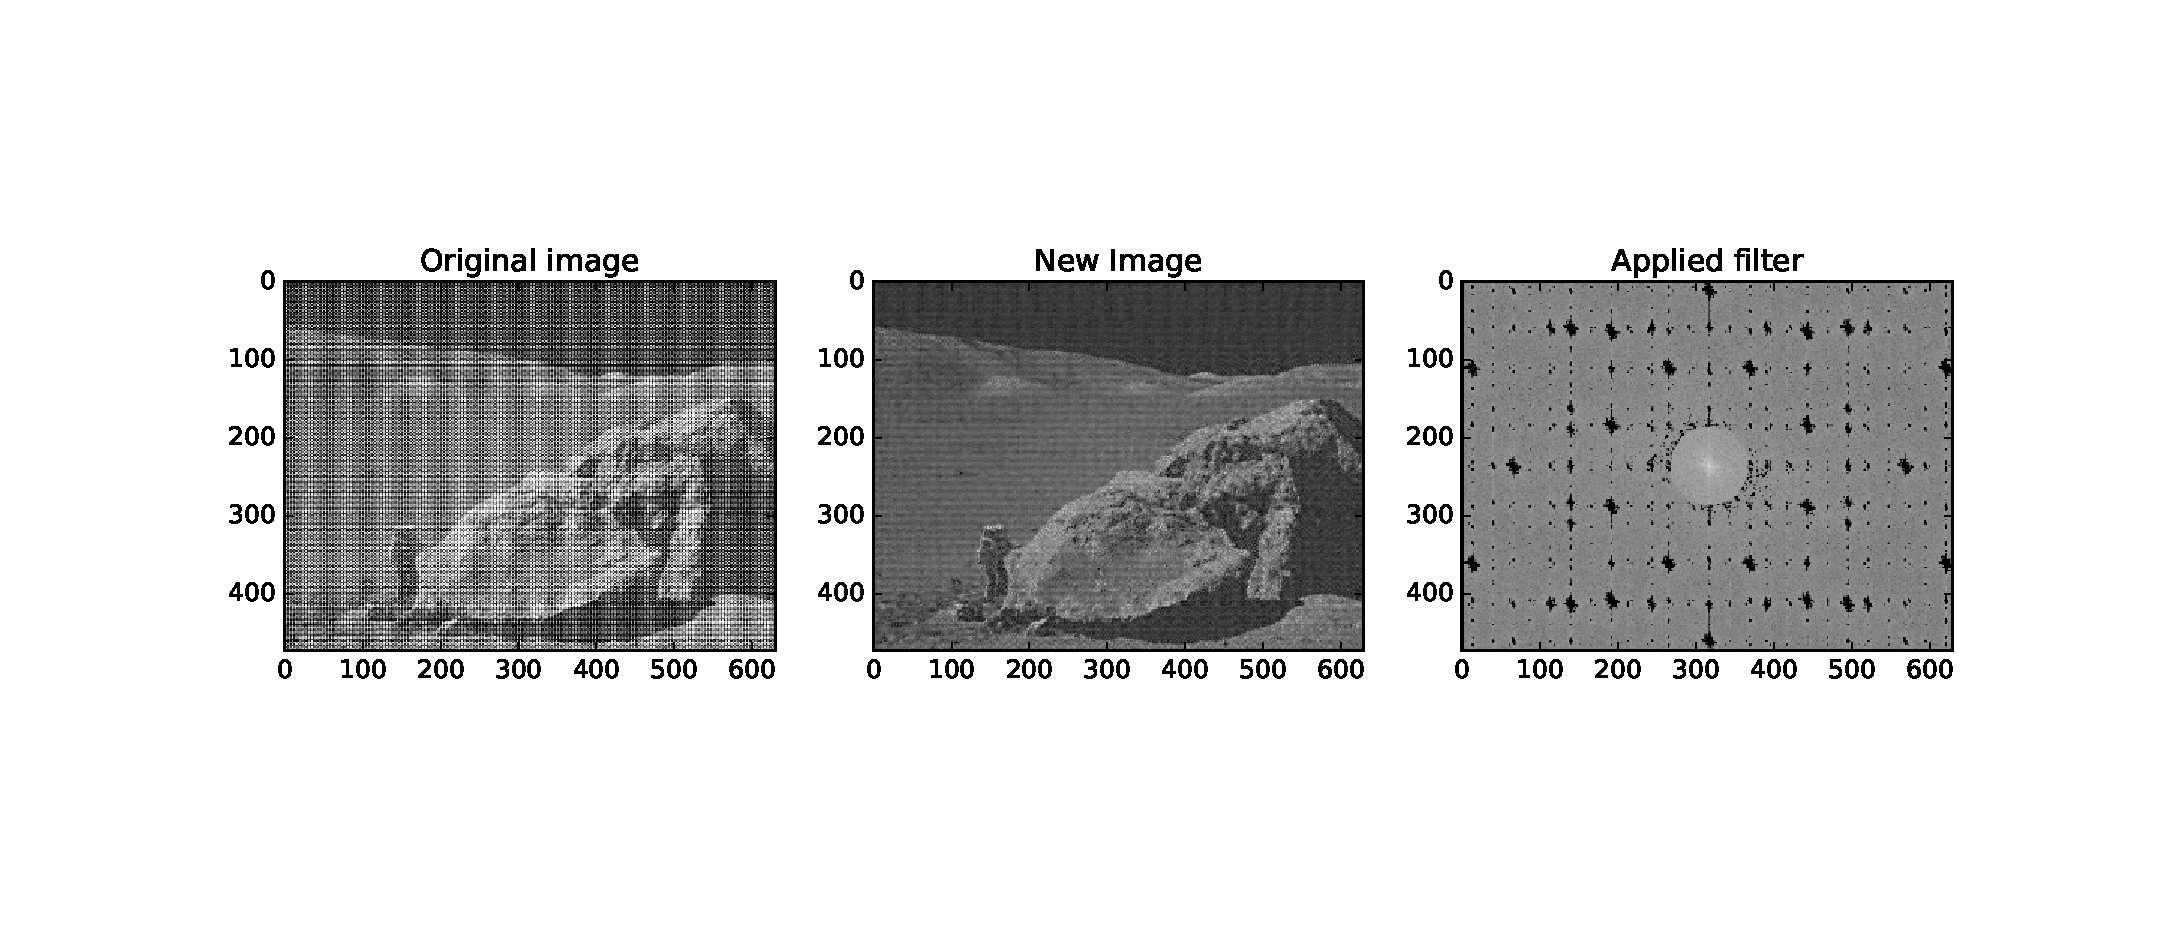
\includegraphics[width=1\linewidth,clip,trim={650 110 75 110}]{pics/moon_fltr_spot}
	\caption{High Energy Spot Filter}
	\label{fig:fltr_spot}
\end{minipage}
\end{figure}







\section{High/Low Pass Filter Kernels}
For high-pass and low-pass filters I've implemented the three main kernels as
previously created in Matlab functions by the Department of Computer Science at
UC Regina\cite{ucr_dftuv,ucr_lpfilter,ucr_hpfilter}. The three kernels they have
implemented in Matlab are "Ideal", "Gaussian" and "Butterworth".  This program
has utilised their Matlab code and ported it to Python\cite{git}, giving us the
following filters below, represented in the form of low pass filters.

As shown in figure \ref{fig:kernel_ideal} the ideal low-pass kernel is binary
based and instantaneously drops from 1 to 0 at the cut-off frequency.  In
perspective the Gaussian kernel, figure \ref{fig:kernel_gaussian}, with same
cut-off frequency has a smoother curve for implementing the filter which smooths
the resulting image.  The Butterworth kernel has an even smoother cut-off curve
as shown in \ref{fig:kernel_btw} resulting in an even smoother low-pass image
when reconstructing the original image from the Fourier transform.

\begin{figure}[h]
\begin{minipage}{0.33\linewidth}
	\centering
	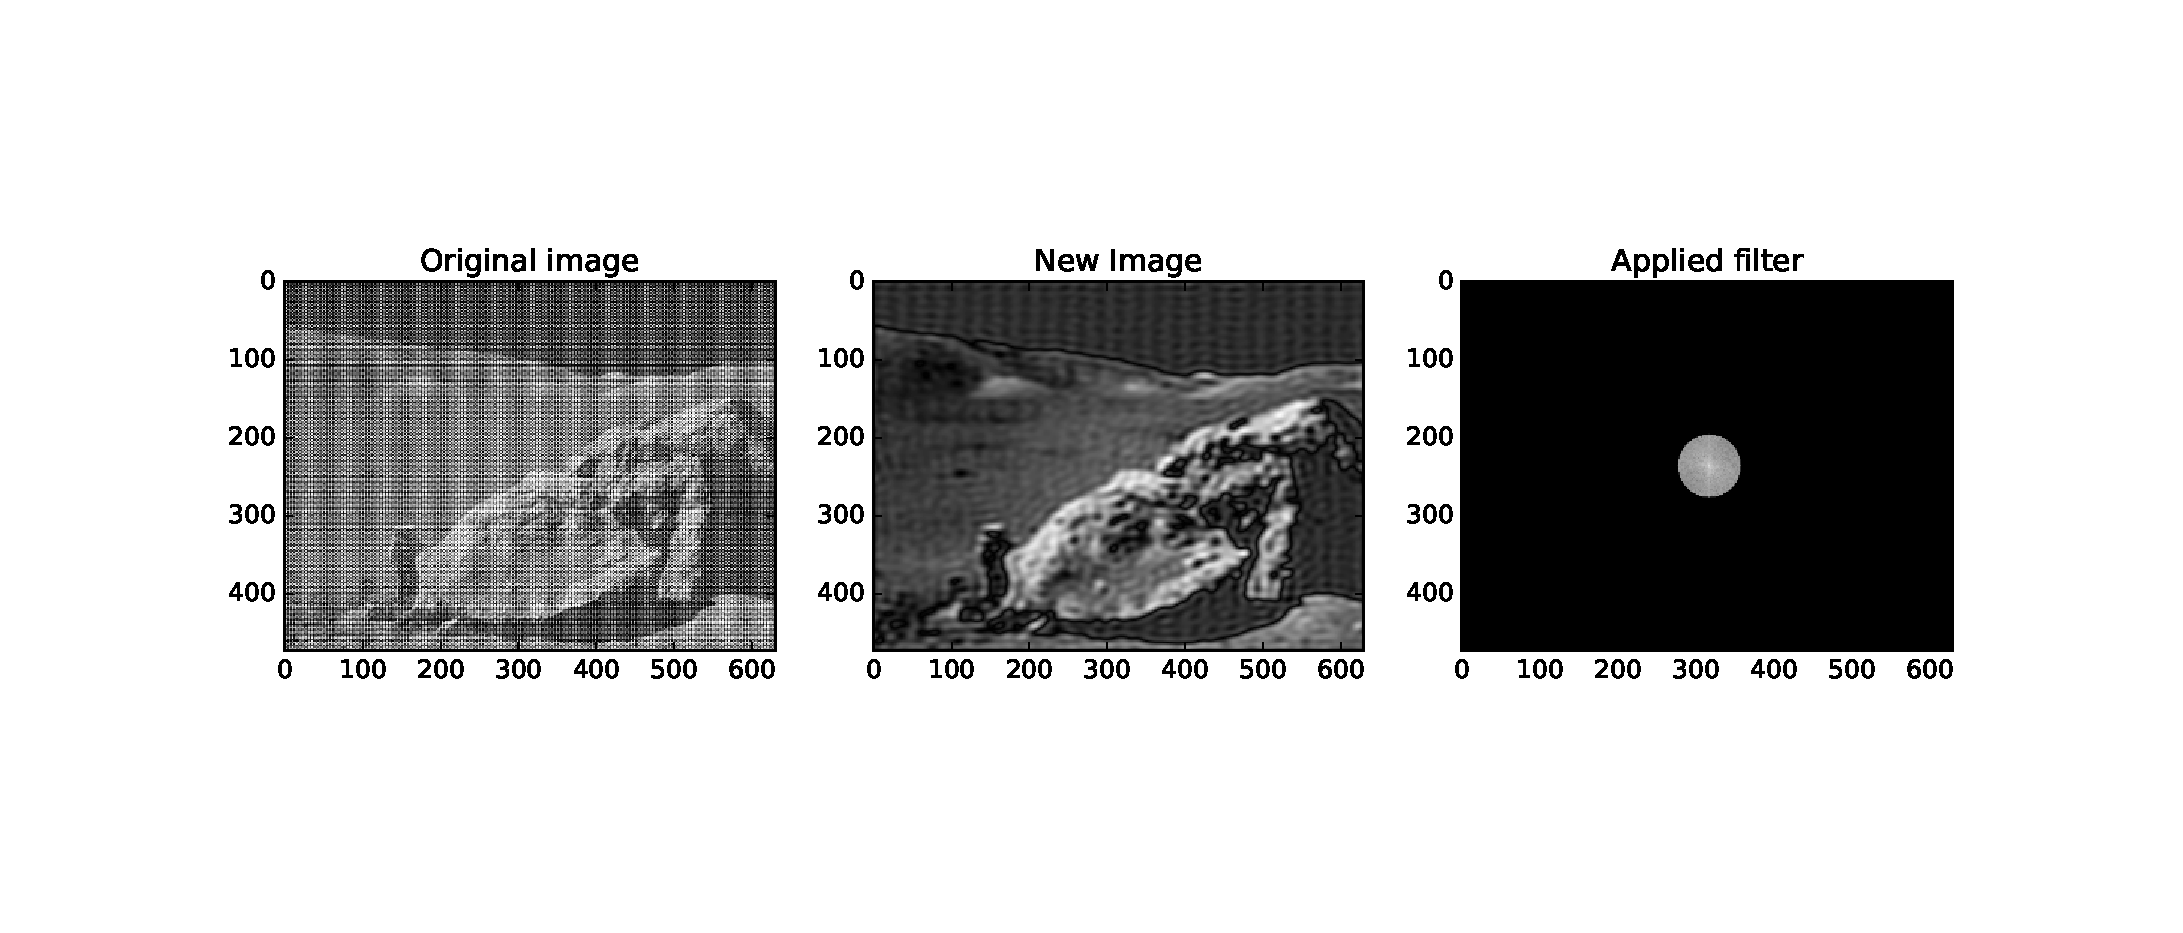
\includegraphics[width=1\linewidth,clip,trim={650 110 75 110}]{pics/moon_lp_ideal}
	\caption{Low pass filter kernel using the ideal method}
	\label{fig:kernel_ideal}
\end{minipage}\hfill
\begin{minipage}{0.33\linewidth}
	\centering
	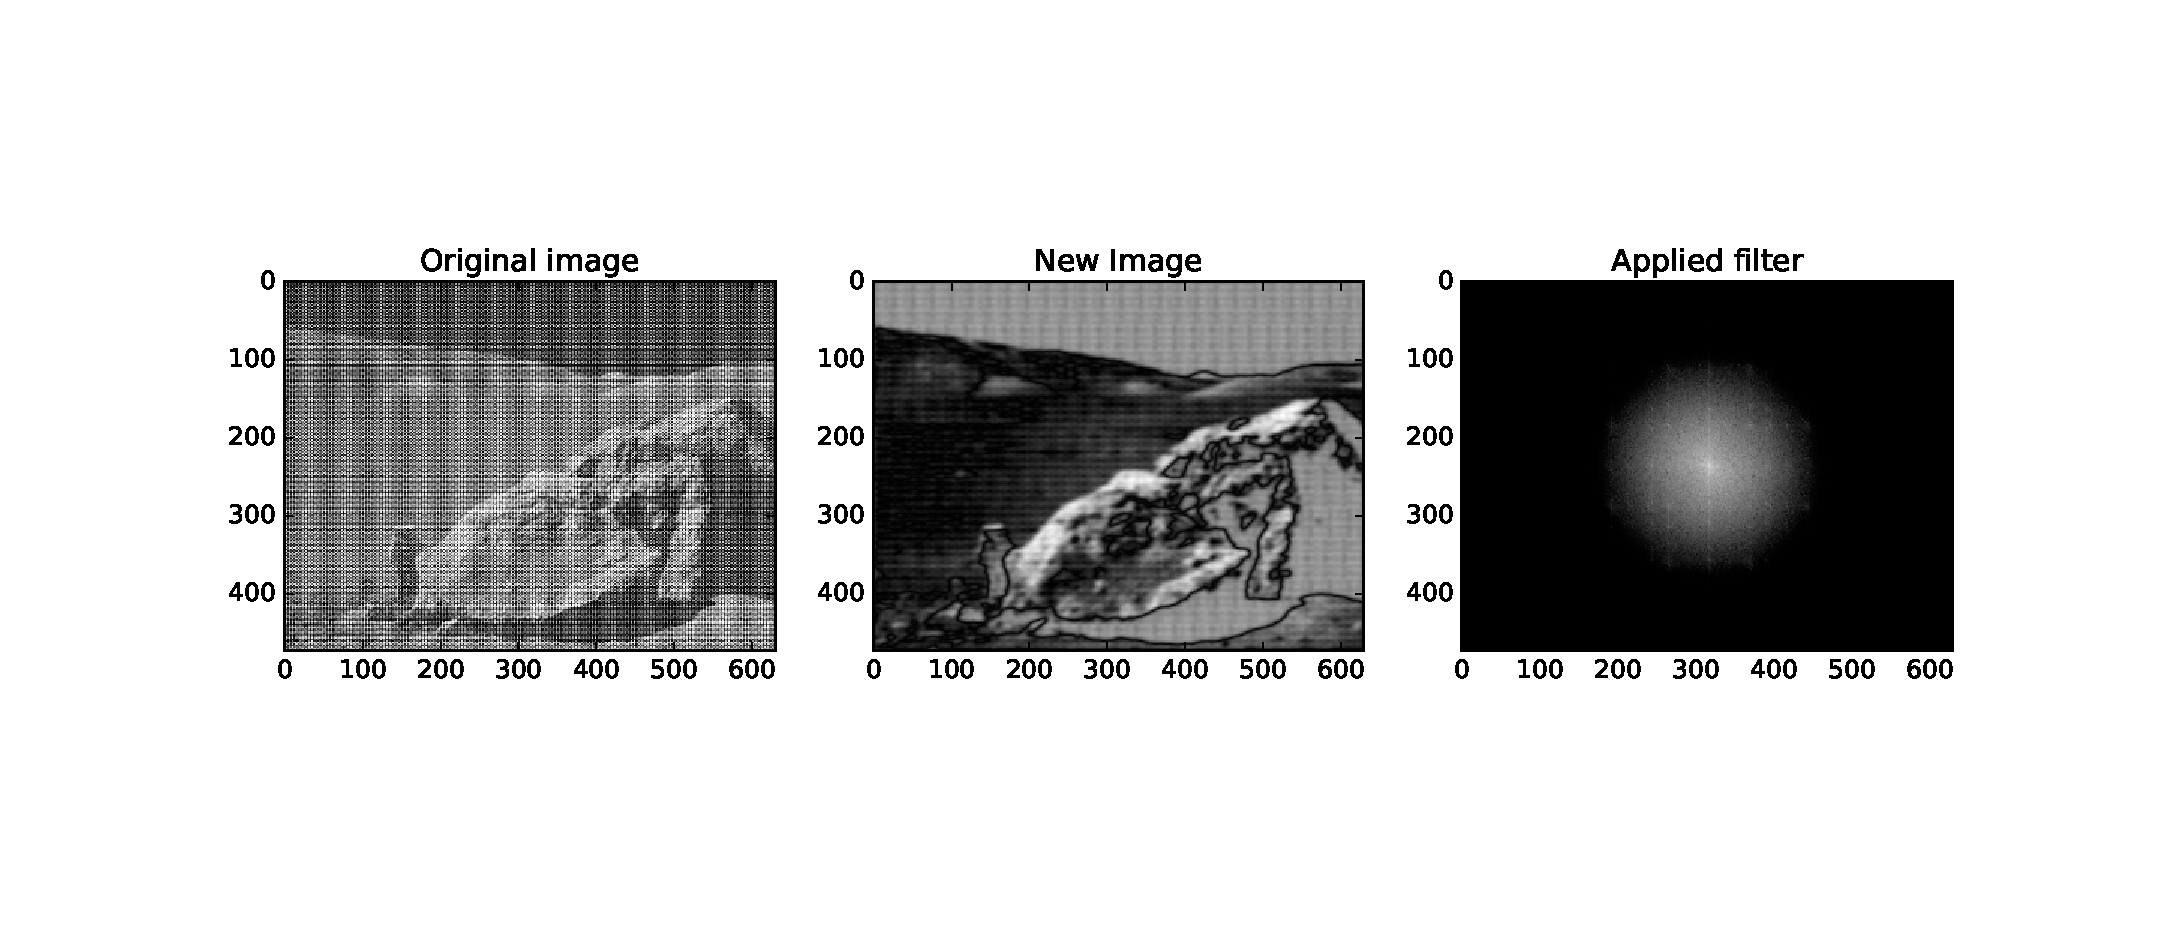
\includegraphics[width=1\linewidth,clip,trim={650 110 75 110}]{pics/moon_lp_gaussian}
	\caption{Low pass filter kernel using the Gaussian equation}
	\label{fig:kernel_gaussian}
\end{minipage}\hfill
\begin{minipage}{0.33\linewidth}
	\centering
	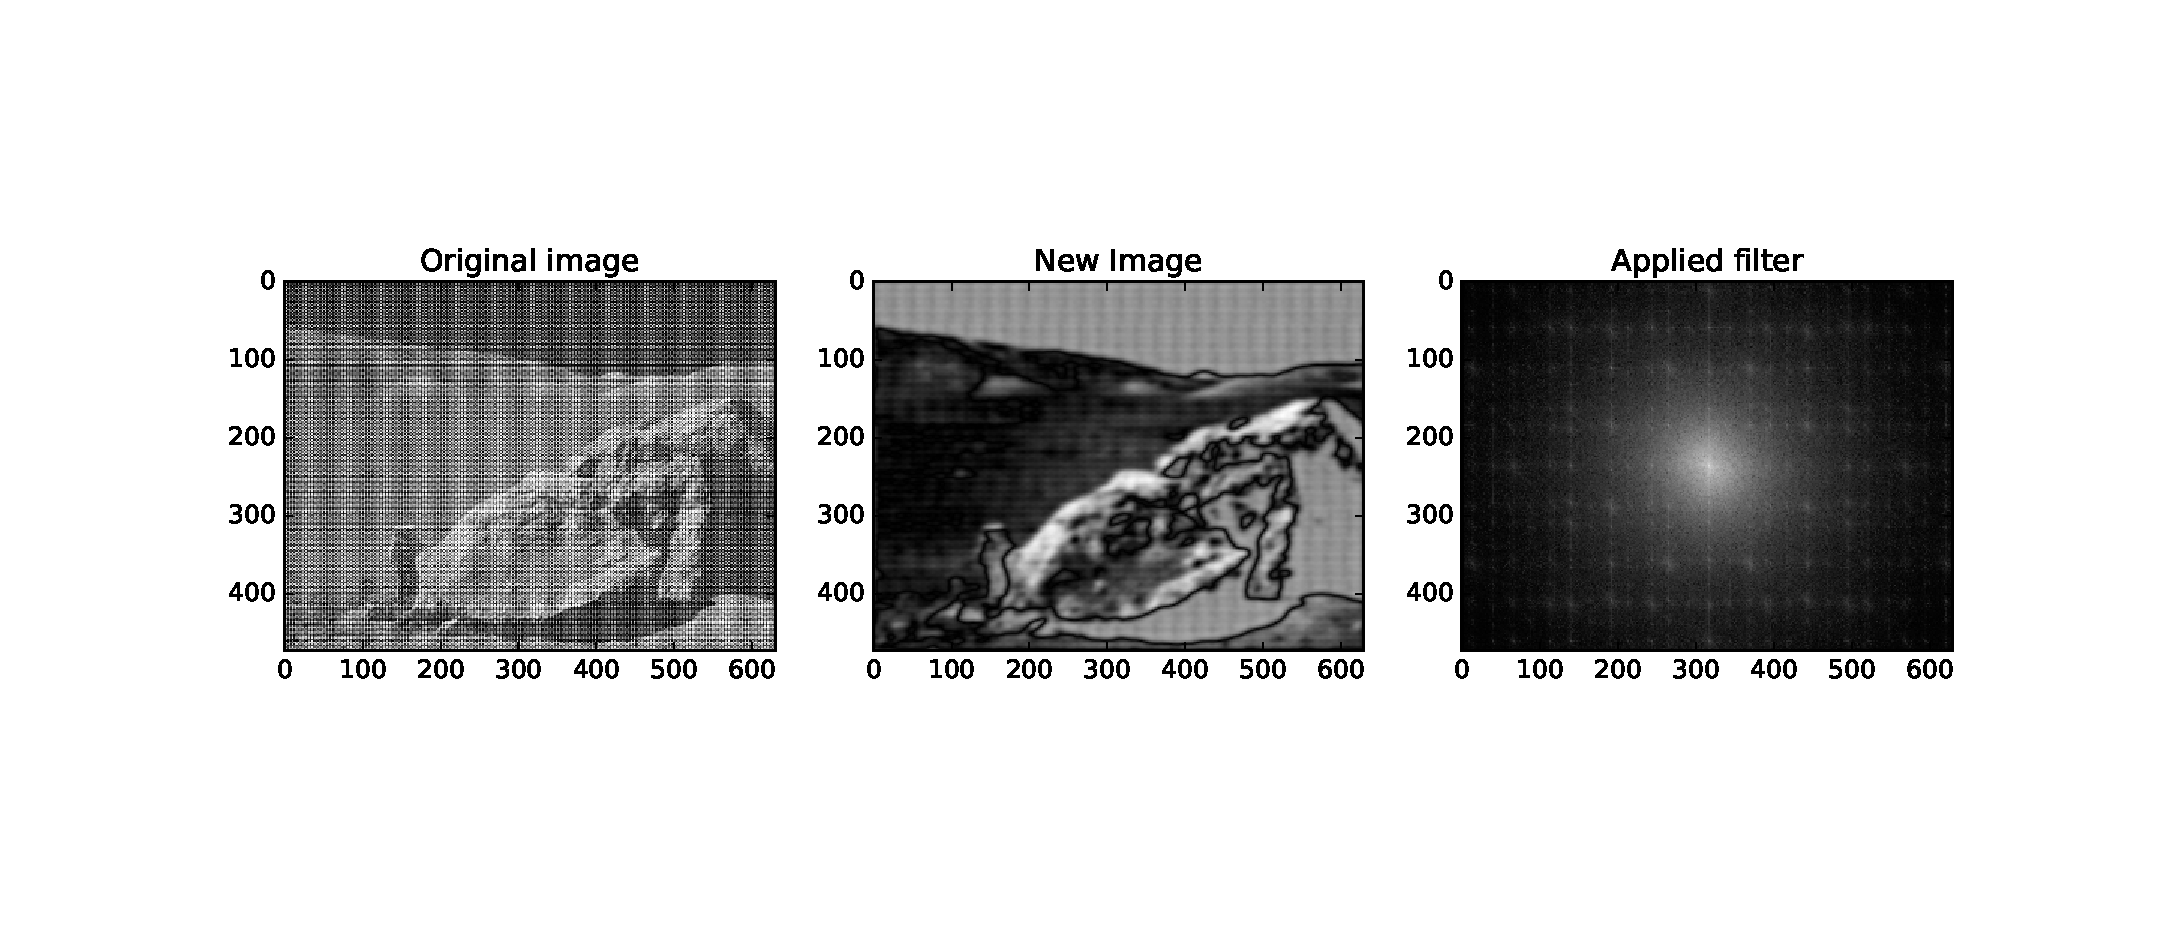
\includegraphics[width=1\linewidth,clip,trim={650 110 75 110}]{pics/moon_lp_btw}
	\caption{Low Pass filter kernel using the Butterworth equation}
	\label{fig:kernel_btw}
\end{minipage}
\end{figure}


